\chapter{СОСТАВЛЕНИЕ МАТЕМАТИЧЕСКОЙ МОДЕЛИ ПНЕВМОПРИВОДА}\label{ch:ch2}
Данная глава посвящена математическому моделированию ПП
с дискретными распределителями. Рассматриваются следующие ключевые аспекты:

\begin{enumerate}
    \item Структура и принцип работы исследуемого ПП;
    \item Моделирование пневмоцилиндра;
    \item Моделирование дискретных распределителей;
    \item Моделирование силы трения и упругих деформаций;
    \item Адаптация математической модели к эффективному численному расчету на ЭВМ.
    \item Верификация математической модели.
\end{enumerate}

Математическая модель включает:

\begin{enumerate}
    \item Уравнения движения поршня;
    \item Уравнения изменения давления в полостях цилиндра;
    \item Уравнения изменения температуры рабочего тела в полостях цилиндра;
    \item Модель массового расхода воздуха;
    \item Модель динамики распределителей;
    \item Модель сил трения;
    \item Модель силы реакции опоры.
\end{enumerate}

Используются уравнения термодинамики и газовой динамики. Учитываются нелинейные эффекты:
сжимаемость воздуха, особенности течения через дросселирующие элементы, силы трения и реакции опоры.

Верификация модели проводится путем проверки математической корректности.


\section{Анализ режимов работы электропневмопривода}\label{sec:ch3/sec1}

Функционирование электропневмопривода с дискретными распределителями характеризуется конечным
множеством возможных состояний системы, определяемых комбинациями состояний распределителей.
Математически пространство состояний распределителей может быть представлено как:

\begin{equation}\label{eq:state_space}
	\mathbf{U} = \left\{
	[u_1, u_2, u_3, u_4] | u_i \in {0,1}, i = 1,\dots,4
	\right\},
\end{equation}
где $u_i$ -- состояние i-го распределителя (0 - закрыт, 1 - открыт).

Теоретически система, как описано ранее, допускает $2^4 = 16$ различных комбинаций состояний распределителей.
Однако с учетом физических ограничений и требований безопасности целесообразно использование только определенного
подмножества состояний, формирующих основные режимы работы привода.

Классификация этих режимов представлена в следующей таблице \ref{tab:operation_modes}.

\begin{table}[htbp]
	\centering
	\caption{Режимы работы электропневматического привода с дискретными распределителями}
	\label{tab:operation_modes}
	\small
	\begin{tabular}{lcll}
		\midrule
		\textbf{Режим}           & $[u_1,u_2,u_3,u_4]$ & \textbf{Движение} & \textbf{Динамика} \\
		\midrule
		СиП\textsuperscript{1}   & $[1,0,0,1]$         &
		Макс. положит. ускорение &
		$M\ddot{x} = p_\text{п}F_1 - p_\text{атм}F_2 - R_\text{тр}$                            \\

		СрП\textsuperscript{2}   & $[1,0,0,0]$         &
		Умер. положит. ускорение &
		$M\ddot{x} = p_\text{п}F_1 - p_2F_2 - R_\text{тр}$                                     \\

		СлП\textsuperscript{3}   & $[0,0,0,1]$         &
		Мин. положит. ускорение  &
		$M\ddot{x} = p_1F_1 - p_\text{атм}F_2 - R_\text{тр}$                                   \\

		СиО.\textsuperscript{4}  & $[0,1,1,0]$         &
		Макс. отриц. ускорение   &
		$M\ddot{x} = p_\text{атм}F_1 - p_\text{п}F_2 - R_\text{тр}$                            \\

		СрО\textsuperscript{5}   & $[0,0,1,0]$         &
		Умер. отриц. ускорение   &
		$M\ddot{x} = p_1F_1 - p_\text{п}F_2 - R_\text{тр}$                                     \\

		СлО\textsuperscript{6}   & $[0,1,0,0]$         &
		Мин. отриц. ускорение    &
		$M\ddot{x} = p_\text{атм}F_1 - p_2F_2 - R_\text{тр}$                                   \\

		\hline
		Н                        & $[0,0,0,0]$         &
		Фиксация положения       &
		$M\ddot{x} = p_1F_1 - p_2F_2 - R_\text{тр}$                                            \\
		\midrule
	\end{tabular}
	\begin{tablenotes}
		\scriptsize
		\item[1] СиП -- сильное положительное ускорение
		\item[2] СрП -- среднее положительное ускорение
		\item[3] СлП -- слабое положительное ускорение
		\item[4] СлО -- сильное отрицательное ускорение
		\item[5] СрО -- среднее отрицательное ускорение
		\item[6] СлО -- слабое отрицательное ускорение
		\item[7] Н -- удержание
	\end{tablenotes}
\end{table}

Динамическое поведение электропневматического привода для каждого режима может быть
проанализировано как в пространстве давлений, так и в фазовом пространстве
скорость-положение. Векторное поле в фазовом пространстве описывается системой дифференциальных уравнений:

\begin{equation}
	\begin{cases}
		\dot{x} = v \\
		\dot{v} = \frac{1}{M}(p_1F_1 - p_2F_2 - R_\text{тр}(v))
	\end{cases}
\end{equation}
где $(x,v)$ -- координаты точки в фазовом пространстве.

Для комплексного понимания динамических процессов в пневмоприводе целесообразно рассмотреть
сравнительные характеристики изменения давлений в полостях пневмоцилиндра
при различных режимах работы, представленные на рисунке \ref{fig:pressure_comparison}.
На графиках отображены процессы для положительного перемещения (выдвижения штока),
поскольку для отрицательного перемещения (втягивания штока) динамика является аналогичной с учетом симметрии системы.

\begin{figure}[htbp]
	\centering
	\includegraphics{part3/pressure_dynamics.pdf}
	\caption{Сравнение динамики установления давлений в различных режимах работы:\\
		а) сильное ускорение; б) умеренное ускорение; в) слабое ускорение; г) режим удержания}
	\label{fig:pressure_comparison}
\end{figure}

Представленные характеристик показывает существенное различие в динамике установления давлений для разных режимов работы.

В режиме сильного положительного ускорения [1,0,0,1] наблюдается максимальный
перепад давлений между полостями цилиндра, что подтверждается системой уравнений:

$$\begin{cases}
		\dot{p}_1 = \frac{\gamma RT_1}{V_1(x)}(G_{1,max} - \frac{p_1}{RT_1}F_1\dot{x}) \\
		\dot{p}_2 = \frac{\gamma RT_2}{V_2(x)}(-G_{4,max} + \frac{p_2}{RT_2}F_2\dot{x})
	\end{cases}$$
где $G_{1,max}$ и $G_{4,max}$ -- максимальные массовые расходы через соответствующие распределители.

Характерной особенностью данного режима является быстрый рост давления $p_1$ до величины, близкой к давлению питания
$p_\text{п}$, с одновременным падением давления $p_2$ до атмосферного давления $p_\text{атм}$. Это обеспечивает интенсивный
разгон штока с последующим выходом на установившуюся скорость, что наглядно демонстрируется на
фазовом портрете (рис. \ref{fig:pp_strong_accelration}). Анализ фазового портрета показывает,
что процесс выхода на установившуюся скорость характеризуется движением изображающей
точки по траектории, асимптотически стремящейся к прямой $v = v_\text{уст}$.

\begin{figure}[htbp]
	\centerfloat{
		\hfill
		\subcaptionbox[List-of-Figures entry]{\label{fig:pp_strong_acceleration_positive}}{
			\includegraphics{part3/pp_strong_acceleration_positive.pdf} }
		\hfill
		\subcaptionbox{\label{fig:pp_strong_acceleration_negative}}{
			\includegraphics{part3/pp_strong_acceleration_negative.pdf} }
	}
	\caption{Фазовые портреты для режима сильного ускорения:\\
		а) положительное ускорение; б) отрицательное ускорение}
	\label{fig:pp_strong_accelration}
\end{figure}

В режимах умеренного ускорения [1,0,0,0]
наблюдается более сложная динамика, обусловленная асимметричным изменением давлений.
При данном режиме динамика давлений описывается системой:

\begin{equation}
	\begin{cases}
		\dot{p}_1 = \frac{\gamma RT_1}{V_1(x)}(G_{1,max} - \frac{p_1}{RT_1}F_1\dot{x}) \\
		\dot{p}_2 = -\frac{\gamma p_2}{V_2(x)}F_2\dot{x}
	\end{cases}
\end{equation}

Особенность данного режима заключается в том, что давление в штоковой полости изменяется согласно политропному процессу:

\begin{equation}
	p_2V_2(x)^n = p_{2,0}V_{2,0}^n = \text{const}
\end{equation}
где $p_{2,0}$ и $V_{2,0}$ -- начальное давление и объем штоковой полости соответственно в момент запирания полости;
$n$ - показатель политропы.

На фазовых портретах представленных на рисунке \ref{fig:pp_moderate_position_1} и рисунке \ref{fig:pp_moderate_position_2}
отчетливо видно влияние начальных условий на динамику системы. При большем начальном положении штока ($x_0$ равное 0,2~\si{\metre}) наблюдается более
интенсивное торможение вследствие меньшего начального объема запертой полости и, соответственно, более быстрого роста давления при сжатии воздуха.

\begin{figure}[htbp]
	\centerfloat{
		\hfill
		\subcaptionbox[List-of-Figures entry]{\label{fig:pp_medium_acceleration_x_01}}{
			\includegraphics{part3/pp_medium_acceleration_x_01.pdf} }
		\hfill
		\subcaptionbox{\label{fig:pp_medium_acceleration_x_01_scheme}}{
			\raisebox{0.5\height}{\includegraphics{part3/pp_medium_acceleration_x_01_scheme.eps}} }
	}
	\caption{Фазовый портрет и схема пневмоцилиндра при начальном положении штока $x_0 = \num{0.1}$ м ($p_{2,0} = p_\text{атм}$):\\
		а) фазовый портрет; б) схема пневмоцилиндра}
	\label{fig:pp_moderate_position_1}
\end{figure}

\begin{figure}[htbp]
	\centerfloat{
		\hfill
		\subcaptionbox[List-of-Figures entry]{\label{fig:pp_medium_acceleration_x_02}}{
			\includegraphics{part3/pp_medium_acceleration_x_02.pdf} }
		\hfill
		\subcaptionbox{\label{fig:pp_medium_acceleration_x_02_scheme}}{
			\raisebox{0.5\height}{\includegraphics{part3/pp_medium_acceleration_x_02_scheme.eps}} }
	}
	\caption{Фазовый портрет и схема пневмоцилиндра при начальном положении штока $x_0 = \num{0.2}$ м ($p_{2,0} = p_\text{атм}$):\\
		а) фазовый портрет; б) схема пневмоцилиндра}
	\label{fig:pp_moderate_position_2}
\end{figure}

Для более полного понимания влияния начальных условий на динамику системы рассмотрена серия фазовых
портретов при различных комбинациях начального положения штока и давления в запираемой
полости (рис. \ref{fig:pp_moderate_matrix}). Анализ данных портретов демонстрирует, что при
фиксированном начальном положении увеличение давления $p_{2,0}$ приводит к снижению установившейся скорости
движения и увеличению интенсивности торможения. При фиксированном начальном давлении
увеличение координаты $x_0$ вызывает сокращение области достижимых состояний и смещение точки остановки к начальному положению.

\begin{figure}[htbp]
	\centerfloat{
		\hfill
		\subcaptionbox[List-of-Figures entry]{\label{fig:pp_medium_acceleration_x_01_p_2}}{
			\includegraphics{part3/pp_medium_acceleration_x_01_p_2.pdf} }
		\hfill
		\subcaptionbox{\label{fig:pp_medium_acceleration_x_01_p_4}}{
			\includegraphics{part3/pp_medium_acceleration_x_01_p_4.pdf}}
		\hfill
		\subcaptionbox{\label{fig:pp_medium_acceleration_x_02_p_2}}{
			\includegraphics{part3/pp_medium_acceleration_x_02_p_2.pdf}}
		\hfill
		\subcaptionbox{\label{fig:pp_medium_acceleration_x_02_p_3}}{
			\includegraphics{part3/pp_medium_acceleration_x_02_p_4.pdf}}
	}
	\caption{Фазовые портреты при различных начальных условиях: \\
		а) $x_0 = \num{0,1}$ м, $p_{2,0} = 2$ бар; б) $x_0 = \num{0.1}$ м, $p_{2,0} = 4$ бар; \\
		в) $x_0 = \num{0.2}$ м, $p_{2,0} = 2$ бар; г) $x_0 = \num{0.2}$ м, $p_{2,0} = 4$ бар;
	}
	\label{fig:pp_moderate_matrix}
\end{figure}

Математически наблюдаемые эффекты описываются уравнением баланса сил:

\begin{equation}
	p_\text{п}F_1 - p_{2,0}\left(\frac{V_{2,0}}{V_2(x)}\right)^nF_2 = R_\text{тр}(v),
\end{equation}
где $V_2(x) = V_{2,0} + A_2(L - x)$ -- текущий объем запертой полости.

Режимы слабого ускорения [0,0,0,1] или [0,1,0,0] характеризуются минимальным перепадом давлений между
полостями пневмоцилиндра. Рассмотрим режим слабого положительного ускорения [0,0,0,1], при котором поршневая полость
изолирована, а штоковая соединена с атмосферой. Динамика давлений в данном режиме описывается системой уравнений:

$$\begin{cases}
		\dot{p}_1 = -\frac{\gamma p_1}{V_1(x)}F_1\dot{x} \\
		\dot{p}_2 = \frac{\gamma RT_2}{V_2(x)}(-G_{4,max} + \frac{p_2}{RT_2}F_2\dot{x})
	\end{cases}$$

На графиках отображенных на рисунке \ref{fig:pressure_comparison} видно, что давление $p_2$ снижается до
тмосферного значения существенно медленнее, чем в режиме сильного ускорения, в то время как
давление $p_1$ изменяется только за счет изменения объема поршневой полости. Данный процесс
характеризуется политропным изменением состояния воздуха в запертой полости:

\begin{equation}
	p_1V_1(x)^n = p_{1,0}V_{1,0}^n = \text{const}
\end{equation}
где $p_{1,0}$ и $V_{1,0}$ -- начальные значения давления и объема поршневой полости соответственно.

\begin{figure}[htbp]
	\centerfloat{
		\hfill
		\subcaptionbox[List-of-Figures entry]{\label{fig:pp_weak_acceleration_x01}}{
			\includegraphics{part3/pp_slow_acceleration_x_01_p_3.pdf} }
		\hfill
		\subcaptionbox{\label{fig:pp_weak_acceleration_x02}}{
			\includegraphics{part3/pp_slow_acceleration_x_02_p_3.pdf} }
	}
	\caption{Фазовые портреты для режима слабого ускорения при различных начальных условиях:\\
		а) $x_0 = \num{0.1}$ м, $p_{1,0} = 3$ бар; б) $x_0 = \num{0.2}$ м, $p_{1,0} = 3$ бар}
	\label{fig:pp_weak_acceleration}
\end{figure}

Анализ фазовых портретов представленных на рисунке \ref{fig:pp_weak_acceleration} показывает существенное влияние начального
положения штока на динамику системы. При увеличении начальной координаты $x_0$ наблюдается снижение максимально достижимой
скорости и уменьшение пути перемещения до точки остановки. Это объясняется более быстрым падением давления $p_1$ при расширении
воздуха в запертой полости большего начального объема.

Уравнение баланса сил для данного режима имеет вид:

\begin{equation}
	p_{1,0}\left(\frac{V_{1,0}}{V_1(x)}\right)^nF_1 - p_\text{атм}F_2 = R_\text{тр}(v)
\end{equation}

где $V_1(x) = V_{1,0} + A_1x$ - текущий объем поршневой полости.

Характерной особенностью режима слабого ускорения является существенная зависимость динамики
от сил трения. На фазовых портретах это проявляется в виде более крутых траекторий
торможения и меньшей области достижимых состояний по сравнению с режимами сильного и
умеренного ускорения. Данный эффект объясняется тем, что движущая сила, определяемая
разностью давлений в полостях, сопоставима по величине с силами трения.

Для оценки влияния начального давления в запертой полости на динамику системы рассмотрим
серию фазовых портретов при различных значениях $p_{1,0}$ приведенных на рисунке \ref{fig:pp_weak_pressure_matrix}.

\begin{figure}[htbp]
	\centerfloat{
		\hfill
		\subcaptionbox[List-of-Figures entry]{\label{fig:pp_weak_p2}}{
			\includegraphics{part3/pp_slow_acceleration_x_015_p_2.pdf} }
		\hfill
		\subcaptionbox{\label{fig:pp_weak_p3}}{
			\includegraphics{part3/pp_slow_acceleration_x_015_p_3.pdf} }
		\vfill
		\subcaptionbox{\label{fig:pp_weak_p4}}{
			\includegraphics{part3/pp_slow_acceleration_x_015_p_4.pdf} }
	}
	\caption{Фазовые портреты при $x_0 = \num{0.15}$ м и различных начальных давлениях:\\
		а) $p_{1,0} = 2$ бар; б) $p_{1,0} = 3$ бар; в) $p_{1,0} = 4$ бар}
	\label{fig:pp_weak_pressure_matrix}
\end{figure}

Анализ представленных фазовых портретов демонстрирует, что увеличение начального давления $p_{1,0}$ приводит
к возрастанию максимальной скорости движения и увеличению дальности перемещения штока. При этом форма
фазовых траекторий становится более пологой, что свидетельствует о меньшем влиянии сил трения
на динамику системы. Данный эффект объясняется увеличением движущей силы при сохранении характера
её изменения в процессе движения.

%%%%%%%%%%%%%%%%%%%%%%%% mode 0

Режим удержания [0,0,0,0] представляет особый интерес с точки зрения
динамики электропневматического привода, поскольку в данном режиме обе полости
пневмоцилиндра оказываются изолированными.Изменение давлений при этом
происходит исключительно за счет изменения объемов полостей и описывается системой уравнений:

$$\begin{cases}
		\dot{p}_1 = -\frac{\gamma p_1}{V_1(x)}F_1\dot{x} \\
		\dot{p}_2 = -\frac{\gamma p_2}{V_2(x)}F_2\dot{x}
	\end{cases}$$

На графиках изменения давлений, согласно рисунку \ref{fig:pressure_comparison}, наблюдается характерное
политропное изменение состояния воздуха в обеих полостях, описываемое уравнениями:

\begin{equation}
	\begin{cases}
		p_1V_1(x)^n = p_{1,0}V_{1,0}^n = \text{const} \\
		p_2V_2(x)^n = p_{2,0}V_{2,0}^n = \text{const}
	\end{cases}
\end{equation}

где $p_{1,0}$, $V_{1,0}$ и $p_{2,0}$, $V_{2,0}$ -- начальные значения давлений и объемов поршневой и штоковой полостей соответственно.

Стабилизация положения штока в режиме удержания обеспечивается преимущественно силами трения, а также дополнительно
поддерживается пневматической жёсткостью, создаваемой сжатым воздухом в изолированных полостях. Баланс сил в данном режиме описывается уравнением:

\begin{equation}
	p_1F_1 - p_2F_2 = R_\text{тр}(v)
\end{equation}

\begin{figure}[htbp]
	\centerfloat{
		\hfill
		\subcaptionbox[List-of-Figures entry]{\label{fig:pp_hold_low_pressure}}{
			\includegraphics{part3/pp_hold_low_pressure.pdf} }
		\hfill
		\subcaptionbox{\label{fig:pp_hold_high_pressure}}{
			\includegraphics{part3/pp_hold_high_pressure.pdf} }
	}
	\caption{Фазовые портреты для режима удержания при различных начальных давлениях:\\
		а) низкие начальные давления ($p_{1,0} = 2$ бар, $p_{2,0} = \num{2}$ бар);\\
		б) высокие начальные давления ($p_{1,0} = 4$ бар, $p_{2,0} = \num{4}$ бар)}
	\label{fig:pp_hold_mode}
\end{figure}

Анализ фазовых портретов для режима удержания показанных на рисунке \ref{fig:pp_hold_mode} показывает высокую эффективность удержания положения штока при различных начальных давлениях.
В системе наблюдается апериодический характер движения с быстрым затуханием скорости, что обусловлено существенным влиянием сил трения.
При этом уровень начальных давлений в полостях оказывает незначительное влияние на характер переходного процесса, что подтверждается схожей формой фазовых траекторий.

\begin{figure}[htbp]
	\centerfloat{
		\hfill
		\subcaptionbox[List-of-Figures entry]{\label{fig:pp_hold_balanced}}{
			\includegraphics{part3/pp_hold_balanced.pdf} }
		\hfill
		\subcaptionbox{\label{fig:pp_hold_unbalanced}}{
			\includegraphics{part3/pp_hold_unbalanced.pdf} }
	}
	\caption{Фазовые портреты при $x_0 = \num{0.15}$ м и различных соотношениях начальных давлений:\\
		а) близкие давления ($p_{1,0} = 3$ бар, $p_{2,0} = 3$ бар);\\
		б) существенная разница ($p_{1,0} = 2$ бар, $p_{2,0} = 4$ бар)}
	\label{fig:pp_hold_matrix}
\end{figure}

Рассмотрение фазовых портретов при различных соотношениях начальных давлений отображенных на  рисунке \ref{fig:pp_hold_matrix} демонстрирует,
что даже при значительной разнице давлений в полостях система сохраняет устойчивое апериодическое движение к положению равновесия.
При близких значениях давлений $p_{1,0}$ и $p_{2,0}$ наблюдается симметричный характер фазовых траекторий. Увеличение разности давлений приводит к незначительной асимметрии траекторий при сохранении общего характера движения.

Математическое описание движения в окрестности положения равновесия может быть получено линеаризацией уравнений движения:

\begin{equation}
	M\ddot{x} + \left(\frac{\gamma p_{1,0}F_1^2}{V_{1,0}} + \frac{\gamma p_{2,0}F_2^2}{V_{2,0}}\right)x + \nu\dot{x} = 0
\end{equation}

где $\nu$ -- коэффициент вязкого трения. Существенное преобладание силы трения над пневматической жёсткостью
($\nu \gg \sqrt{M\left(\frac{\gamma p_{1,0}F_1^2}{V_{1,0}} + \frac{\gamma p_{2,0}F_2^2}{V_{2,0}}\right)}$) обуславливает апериодический характер движения системы.

Проведенный анализ режимов работы электропневматического привода с дискретными распределителями
позволил выявить характерные особенности динамики системы для каждого режима функционирования.
В режиме сильного ускорения [1,0,0,1] наблюдается максимальный перепад давлений между полостями и,
как следствие, наибольшая интенсивность разгона штока с последующим выходом на установившуюся скорость.
Режим умеренного ускорения [1,0,0,0] характеризуется существенным влиянием начальных условий на динамику
системы вследствие политропного изменения состояния воздуха в запертой полости. Режим слабого ускорения
[0,0,0,1] демонстрирует значительную зависимость от сил трения при минимальном перепаде давлений между полостями.
Особую роль играет режим удержания [0,0,0,0], в котором стабилизация положения штока обеспечивается преимущественно
силами трения при апериодическом характере затухания скорости. Построенные фазовые портреты и анализ динамики давлений
позволяют обоснованно подходить к выбору режимов работы при проектировании алгоритмов управления электропневматическим
приводом с дискретными распределителями. При этом учет выявленных закономерностей и особенностей каждого режима позволяет
обеспечить требуемые показатели качества позиционирования при минимизации количества переключений распределителей.
\section{Постановка задачи многокритериальной оптимизации параметров пневмопривода}\label{ch:ch4/sec2}

Для решения задачи применяются методы построения фронта Парето,
позволяющие выделить множество неулучшаемых решений, представляющих
компромисс между критериями. Оптимизационная задача формулируется как
поиск таких значений параметров управления, при которых улучшается
один из критериев, не ухудшая при этом другие. Это достигается путем
численного моделирования системы с использованием суррогатных моделей,
которые сокращают вычислительные затраты и позволяют быстро оценивать
показатели качества при различных сочетаниях параметров. Результаты
оптимизации используются для выбора наилучшей стратегии управления
пневмоприводом в зависимости от заданных условий эксплуатации и
требований к точности и ресурсам системы.

\subsection{Концепция оптимальности по Парето}\label{ch:ch4/sec2/subsec1}

Концепция оптимальности по Парето, предложенная итальянским экономистом
Вильфредо Парето \cite*{pareto1896cours} в конце XIX века, является фундаментальным понятием в теории
многокритериальной оптимизации. Данная концепция предоставляет математический аппарат для
анализа и принятия решений \cite*{miettinen1999nonlinear} в ситуациях, где необходимо одновременно оптимизировать несколько,
зачастую противоречивых, критериев.

Рассмотрим задачу многокритериальной оптимизации с $k$ целевыми функциями \cite*{deb2001multi}:

\begin{equation}
    \label{eq:multiobjective_optimization}
    \min_{x \in \Omega} F(x) = (\min f_1(x), \min f_2(x), \ldots, \min f_k(x)),
\end{equation}
где $x \in \Omega \subset \mathbb{R}^n$ -- вектор решений, принадлежащий допустимому множеству $\Omega$;
$F: \Omega \rightarrow \mathbb{R}^k$ -- векторная целевая функция.

Решение $x^* \in \Omega$ называется оптимальным по Парето
(или Парето-оптимальным), если не существует другого решения $x \in \Omega$, такого что:

\begin{equation}
    \begin{cases}
        \forall i \in \{1, \ldots, k\}: f_i(x) \leq f_i(x^*), \\
        \exists j \in \{1, \ldots, k\}: f_j(x) < f_j(x^*).
    \end{cases}
\end{equation}

Иными словами, решение является Парето-оптимальным, если невозможно
улучшить значение любого критерия без ухудшения значения хотя бы одного другого критерия.

Концепция оптимальности по Парето тесно связана с понятием доминирования.
Говорят, что решение $x_1$ доминирует решение $x_2$ (обозначается как $x_1 \prec x_2$), если выполняются следующие условия:

\begin{equation}
    \label{eq:dominance}
    \begin{cases}
        \forall i \in \{1, \ldots, k\}: f_i(x_1) \leq f_i(x_2), \\
        \exists j \in \{1, \ldots, k\}: f_j(x_1) < f_j(x_2).
    \end{cases}
\end{equation}

Множество всех Парето-оптимальных решений образует множество
недоминируемых решений, которое также называется множеством Парето или Парето-множеством.

Образ множества Парето в пространстве критериев называется фронтом Парето. Математически фронт Парето можно определить как:

\begin{equation}
    PF = \{F(x) | x \in PS\},
\end{equation}
где $PS$ -- множество Парето в пространстве решений.

Фронт Парето представляет собой геометрическое место точек \cite*{coello2007evolutionary} в
пространстве критериев, соответствующих недоминируемым решениям.
Он наглядно демонстрирует компромиссы между различными целевыми
функциями и играет ключевую роль в процессе принятия решений.

На рисунке \ref{fig:pareto_front_example} приведен пример фронта Парето для двух критериев.

\begin{figure}[ht]
    \centerfloat{
    \includegraphics{part4/pareto_front_demonstrate.pdf}
    }
    \caption{Пример фронта Парето для двух критериев.}\label{fig:pareto_front_example}
\end{figure}[ht]

На рисунке видно, что фронт Парето представляет собой кривую, состоящую из
недоминируемых решений
(точек), для которых невозможно улучшить один критерий без ухудшения другого.

Основные свойства оптимальности по Парето:
\begin{enumerate}
    \item Несравнимость: Парето-оптимальные решения несравнимы между собой в смысле доминирования.

    \item Иерархическая структура: Концепция Парето-оптимальности может быть расширена на случай иерархической оптимизации, где критерии имеют различные приоритеты.

    \item Инвариантность: Парето-оптимальные решения инвариантны относительно монотонных преобразований целевых функций.

    \item Выпуклость: Если все целевые функции выпуклы и допустимое множество выпукло, то множество Парето также выпукло.
\end{enumerate}

Для нахождения множества Парето-оптимальных решений в задачах многокритериальной оптимизации
используются специальные эволюционные алгоритмы. Эти методы работают с популяциями решений и
постепенно улучшают их, используя механизмы, подобные естественному отбору. Ниже описаны два из наиболее
известных алгоритмов для поиска Парето-оптимальных решений.

Сущществует множество методов для поиска Парето-оптимальных решений, однако наиболее
распространенными являются эволюционные алгоритмы, такие как NSGA-II и SPEA2.

NSGA-II — это один из самых популярных эволюционных алгоритмов для многокритериальной оптимизации. Его ключевые особенности:

\begin{enumerate}
    \item Сортировка по доминированию: На каждом шаге алгоритм делит популяцию на несколько уровней,
    исходя из степени доминирования решений. Те решения, которые не доминируются другими, попадают в
    первый уровень, остальные сортируются в соответствии с их степенью доминирования.

    \item Crowding Distance: NSGA-II использует метрику "crowding distance" для оценки плотности
    решений в области фронта Парето. Это помогает поддерживать разнообразие решений, предотвращая
    их слияние в одном месте.

    \item Операторы отбора, скрещивания и мутаций: Алгоритм применяет стандартные операторы
    генетического алгоритма для эволюции популяции — отбор лучших решений, скрещивание и мутацию
    для создания нового поколения.
\end{enumerate}

NSGA-II обеспечивает эффективное нахождение множества Парето-оптимальных решений,
а также хорошо сохраняет разнообразие решений вдоль фронта Парето \cite*{deb2001multi}.

SPEA2 — это улучшенная версия алгоритма SPEA, разработанная для повышения эффективности поиска недоминируемых решений. Основные улучшения SPEA2 включают:

\begin{enumerate}
    \item Архивирование решений: SPEA2 сохраняет архив недоминируемых решений на каждом шаге, что помогает гарантировать,
    что фронт Парето не будет потерян в процессе эволюции.

    \item Оценка решений: Каждый элемент популяции получает оценку на основе того,
    сколько решений он доминирует и насколько сильно доминируется сам. Эта оценка
    используется для выбора кандидатов для следующего поколения.

    \item Учет плотности решений: Подобно NSGA-II, SPEA2 учитывает плотность решений
    вблизи каждого кандидата, что помогает поддерживать разнообразие и улучшать
    распределение решений вдоль фронта Парето.
\end{enumerate}

SPEA2 продемонстрировал высокую производительность на сложных задачах многокритериальной
оптимизации и может эффективно находить множество недоминируемых решений \cite{zitzler2001spea2}.

В задаче оптимизации параметров управления пневматическим приводом концепция оптимальности
по Парето позволяет учесть множественные, зачастую противоречивые, критерии качества управления.
Например, минимизация времени переходного процесса и минимизация колличества переключений распределителей
могут находиться в конфликте друг с другом. Построение фронта Парето в этом случае
позволяет выявить множество оптимальных компромиссных решений и
предоставить лицу, принимающему решения, полную картину возможных вариантов.
\section{Моделирование дискретных распределителей}\label{sec:ch2/sec3}

\subsection{Уравнения массового расхода рабочего тела}\label{sec:ch2/sec3/subsec1}
Массовый расход воздуха через дискретный распределитель
является ключевым параметром, определяющим динамику пневматической
системы. Для его описания используется модель, основанная на уравнении Сен-Венана-Ванцеля:
\begin{equation}
    G = \psi(p_1, p_2) \cdot C_d F_\text{пр} \frac{p_1}{\sqrt{RT_\text{вх}}},
\end{equation}
где
$\psi(p_1, p_2)$ -- расходная функция;
$C_d$ -- коэффициент расхода;
$F_\text{пр}$ -- эффективная площадь проходного сечения;
$p_1$ -- давление на входе;
$p_2$ -- давление на выходе;
$T_\text{вх}$ -- температура воздуха на входе.

Ключевым элементом в данном уравнении является расходная функция $\psi(p_1, p_2)$, которая
учитывает влияние отношения давлений на входе и выходе распределителя
на массовый расход. Эта функция определяется следующим образом:
\begin{equation}
    \psi(p_1, p_2) = \begin{cases}
        \sqrt{\frac{2\gamma}{\gamma-1}\left[\left(\frac{p_2}{p_1}\right)^{\frac{2}{\gamma}} - \left(\frac{p_2}{p_1}\right)^{\frac{\gamma+1}{\gamma}}\right]}, & \text{если } \frac{p_2}{p_1} > b_{кр}    \\
        \sqrt{\gamma \left(\frac{2}{\gamma+1}\right)^{\frac{\gamma+1}{\gamma-1}}},                                                                            & \text{если } \frac{p_2}{p_1} \leq b_{кр}
    \end{cases}
\end{equation}
где
$b_{кр} = \left(\frac{2}{\gamma+1}\right)^{\frac{\gamma}{\gamma-1}}$ -- критическое отношение давлений.

Для наглядного представления характера изменения расходной функции
$\psi(p_1, p_2)$ в зависимости от отношения давлений $p_2/p_1$
приведен график представлены на рисунке \ref{fig:ch2/mass_flow_function}.
\begin{figure}
    \centerfloat{
        \includegraphics{part2/critical_gas_flow_chart.eps}
    }
    \caption{График расходной функции $\psi(p_1, p_2)$}
    \label{fig:ch2/mass_flow_function}
\end{figure}

На графике отчетливо видны две области: докритическое и закритическое течение, разделенные точкой
критического отношения давлений $b_{кр}$.

В области докритического течения ($p_2/p_1 > b_{кр}$) расход зависит от отношения давлений и
описывается нелинейной функцией. Здесь наблюдается плавное увеличение расхода с уменьшением отношения давлений.

В закритической области ($p_2/p_1 \leq b_{кр}$) расход достигает максимального
значения и остается постоянным независимо от дальнейшего снижения отношения давлений.
Это явление связано с достижением скорости потока воздуха
в самом узком сечении распределителя скорости звука.

Критическая точка $b_{кр}$ соответствует условию, при котором скорость потока
воздуха в самом узком сечении распределителя достигает скорости звука. Для
воздуха при нормальных условиях значение $b_{кр}$ составляет приблизительно \num{0.528}.
Эффективная площадь проходного сечения $F_\text{др}$ зависит от
положения запорно-регулирующего элемента распределителя и может
быть представлена как функция управляющего сигнала $u$:
\begin{equation}
    F_\text{др} = F_{max} \cdot f(u),
\end{equation}
где $F_{max} = F_\text{пр}$ -- максимальная эффективная площадь проходного сечения;
$f(u)$ -- функция, описывающая зависимость площади от управляющего сигнала.

В данной работе используется линейная зависимость площади проходного сечения от управляющего сигнала.
\begin{equation}
    f(u) = F_{max} \cdot u.
\end{equation}

Тогда уравнение массового расхода принимает вид:
\begin{equation}
\label{eq:ch2/mass_flow}
    G = \psi(p_1, p_2) \cdot C_d F_{max} \cdot u \frac{p_1}{\sqrt{RT_\text{вх}}}.
\end{equation}

Представленная модель массового расхода позволяет точно описать процесс истечения
воздуха через дискретный распределитель в различных режимах работы
пневмопривода. Учет нелинейного характера расходной функции и
влияния критического отношения давлений особенно важен при анализе динамики
системы и разработке алгоритмов управления, обеспечивающих высокую точность
и быстродействие электропневматического привода.

\subsection{Динамика переключения распределителей}\label{sec:ch2/sec3/subsec2}

Процесс переключения дискретного распределителя характеризуется
определенной динамикой, которую необходимо учитывать для точного моделирования поведения
системы. Динамика переключения может быть описана дифференциальным уравнением первого порядка:
\begin{equation}
\label{eq:ch2/switching_dynamics}
    \tau \frac{du}{dt} + u = u_{зад},
\end{equation}
где:
$u$ -- текущее положение запорно-регулирующего элемента;
$u_{зад}$ -- заданное положение (0 или 1 для дискретного распределителя);
$\tau$ -- постоянная времени переключения.

Учет динамики переключения позволяет моделировать такие эффекты, как задержка
срабатывания и дребезг контактов, которые могут оказывать
существенное влияние на поведение системы,
особенно при высокочастотном управлении.

Интеграция моделей массового расхода и динамики переключения
в общую математическую модель электропневматического привода
осуществляется путем их включения в уравнения
изменения давлений в полостях пневмоцилиндра \ref{eq:ch2/pressure_system}.

В данной работе использована модель первого порядка для описания динамики переключения
поскольку она обеспечивает достаточно точное описание процесса переключения
и имеет простую структуру.



\section{Адаптация математической модели к эффективному численному расчету на ЭВМ}\label{sec:ch2/sec4}

Эффективное численное моделирование динамики электропневматического привода требует
оптимизации математической модели для выполнения расчетов на ЭВМ.
Данный этап критически важен для обеспечения высокой производительности
вычислений при проведении многочисленных итераций в задачах оптимизации,
анализа чувствительности и робастности системы управления.

Основные цели оптимизации математической модели включают:

\begin{enumerate}
    \item Снижение вычислительной сложности уравнений;
    \item Уменьшение времени выполнения расчетов;
    \item Повышение численной устойчивости алгоритмов;
    \item Эффективное использование параллельных вычислительных архитектур.
\end{enumerate}

Для достижения этих целей будут применены следующие методы:

\begin{enumerate}
    \item Векторизация уравнений;
    \item Упрощение и линеаризация нелинейных выражений;
    \item Предварительное вычисление констант и коэффициентов;
\end{enumerate}
\subsection{Векторизация уравнений}\label{sec:ch2/sec4/subsec1}
Векторизация уравнений представляет собой эффективный метод оптимизации вычислений,
позволяющий использовать преимущества SIMD-инструкций (Single Instruction, Multiple Data)
современных процессоров. Данный подход особенно актуален для математической
модели электропневматического привода с дискретными распределителями, где многие операции могут быть выполнены
параллельно \cite*{eichenberger2004simd} над несколькими элементами данных.

Основная идея векторизации заключается в преобразовании скалярных операций в
векторные, что позволяет обрабатывать несколько элементов данных
одновременно \cite*{nuzman2011vaporsimd}. В контексте рассматриваемой модели это означает переход от
поэлементных вычислений к операциям над векторами и матрицами.
Процесс векторизации начинается с представления состояния системы
в виде единого вектора. Для электропневматического привода
вектор состояния может быть записан как:

\begin{equation}
\label{eq:ch2/state_vector}
    \mathbf{y} = [x, v, p_1, p_2, T_1, T_2, u_1, u_2, u_3, u_4]^T.
\end{equation}

Векторизованная форма уравнения движения поршня \eqref{eq:ch2/eq8} может быть представлена следующим образом:

\begin{equation}
\label{eq:ch2/vec_motion}
    M\ddot{x} = \mathbf{F}^T\mathbf{p} - p_\text{атм}(\mathbf{F}^T\mathbf{1}) - R_\text{тр}(\dot{x}) - R_\text{оп}(x, \dot{x}),
\end{equation}
где $\mathbf{F} = [F_1, -F_2]^T$ -- вектор эффективных площадей поршня;
$\mathbf{p} = [p_1, p_2]^T$ -- вектор давлений в полостях цилиндра;
$\mathbf{1} = [1, 1]^T$ - единичный вектор.

Уравнения изменения давлений в полостях \eqref{eq:ch2/final_pressure_system} могут быть векторизованы следующим образом:
\begin{equation}
\label{eq:ch2/vec_pressure}
    \dot{\mathbf{p}} = \frac{\gamma}{\mathbf{V}(\mathbf{x})} \odot (R\mathbf{T} \odot \mathbf{G} - \mathbf{p} \odot (\mathbf{F}\dot{x})),
\end{equation}
где $\odot$ обозначает поэлементное умножение векторов;
$\mathbf{T} = [T_1, T_2]^T$ -- вектор температур в полостях;
$\mathbf{G} = [G_1, G_2]^T$ -- вектор суммарных массовых расходов для каждой полости;
$\mathbf{V}(\mathbf{x}) = [V_1(x), V_2(x)]^T$ -- вектор-функция объемов полостей.

Уравнения изменения температур \eqref{eq:ch2/energy_balance_final} также могут быть представлены в векторной форме:
\begin{equation}
\label{eq:ch2/vec_temperature}
    \dot{\mathbf{T}} = \frac{\gamma-1}{\mathbf{m}C_v} \odot (R\mathbf{T} \odot \mathbf{G} \pm \mathbf{p} \odot (\mathbf{F}\dot{x})),
\end{equation}
где $\mathbf{m} = [m_1, m_2]^T$ -- вектор масс воздуха в полостях.

Динамика переключения распределителей \eqref{eq:ch2/switching_dynamics} может быть векторизована для всех четырех распределителей одновременно:
\begin{equation}
\label{eq:ch2/vec_switching}
    \tau \dot{\mathbf{u}} + \mathbf{u} = \mathbf{u}_\text{зад},
\end{equation}
где $\mathbf{u} = [u_1, u_2, u_3, u_4]^T$ -- вектор текущих положений запорно-регулирующих элементов распределителей;
$\mathbf{u}_\text{зад}$ -- вектор заданных положений.

Для расчета массовых расходов через распределители можно использовать векторизованную форму уравнения массового расхода:
\begin{equation}
\label{eq:ch2/vec_mass_flow}
    \mathbf{G} = \psi(\mathbf{p}_\text{вх}, \mathbf{p}_\text{вых}) \odot \mathbf{C}_d \odot \mathbf{F}_\text{пр} \odot \mathbf{u} \odot \frac{\mathbf{p}_\text{вх}}{\sqrt{R\mathbf{T}_\text{вх}}},
\end{equation}
где $\psi(\mathbf{p}_\text{вх}, \mathbf{p}_\text{вых})$ -- векторизованная расходная функция;
$\mathbf{C}_d$ и $\mathbf{F}_\text{пр}$ -- векторы коэффициентов расхода и эффективных площадей проходных сечений распределителей соответственно.

Применение векторизации позволяет эффективно использовать SIMD-инструкции процессора,
что приводит к значительному ускорению вычислений. В зависимости от архитектуры процессора и
специфики реализации, ускорение может достигать 2-4 раза \cite*{tian2013simd} по сравнению с исходной скалярной версией.

\subsection{Оптимизация нелинейных функций}\label{sec:ch2/sec4/subsec2}

Так же важным этапом оптимизации является упрощение и линеаризация нелинейных функций,
которые могут оказывать существенное влияние на вычислительную сложность модели и деаль ее
жесткой. В контексте электропневматического привода, к нелинейным функцям относятся экспоненциальная
функция в модели трения, функция sign, реакция упоров и условные операции.

Для оптимизации вычисления экспоненциальной функции в модели трения предлагается использовать аппроксимацию Паде.
Данный метод обеспечивает высокую точность аппроксимации при сравнительно низкой вычислительной
сложности. Аппроксимация Паде для экспоненциальной функции может быть представлена в виде:

\begin{equation}
    e^x \approx \frac{1 + \frac{x}{2} + \frac{x^2}{10} + \frac{x^3}{120}}{1 - \frac{x}{2} + \frac{x^2}{10} - \frac{x^3}{120}}.
\end{equation}

Данная аппроксимация обеспечивает высокую точность в диапазоне $x \in [-2,5; 2,5]$,
что достаточно для моделирования эффекта Штрибека в рассматриваемой системе.

Реакция упоров, обычно моделируемая с использованием условных операций, может быть
оптимизирована применением непрерывной аппроксимации:

\begin{equation}
    R_\text{оп} = k_\text{оп}(x - x_\text{мин})\cdot S(x - x_\text{мин}) + k_\text{оп}(x - x_\text{макс})\cdot S(x - x_\text{макс}),
\end{equation}
где $S(x)$ -- сглаживающая функция, например:

\begin{equation}
    S(x) = \frac{1}{1 + e^{-\alpha x}},
\end{equation}
где $\alpha$ -- параметр, определяющий крутизну перехода.

Для оптимизации условных операций в модели предлагается
использовать непрерывные аппроксимации. Например, функция
максимума может быть аппроксимирована как:

\begin{equation}
    \max(a, b) \approx \frac{a + b + \sqrt{(a - b)^2 + \varepsilon}}{2},
\end{equation}
где $\varepsilon$ -- малое положительное число, обеспечивающее гладкость функции.

Применяя предложенные оптимизации, уравнения реакции упоров и силы трения могут быть представлены в виде:

\begin{equation}
    \begin{alignedat}{2}
        g(v) & = \left[R_\text{к} + (R_\text{с} - R_\text{к})\frac{1 + \frac{z}{2} + \frac{z^2}{10} + \frac{z^3}{120}}{1 - \frac{z}{2} + \frac{z^2}{10} - \frac{z^3}{120}}\right] \\
        R_\text{оп} & = k_\text{оп}(x - x_\text{мин})\cdot \frac{1}{1 + e^{-\alpha(x - x_\text{мин})}} + k_\text{оп}(x - x_\text{макс})\cdot \frac{1}{1 + e^{-\alpha(x - x_\text{макс})}},
    \end{alignedat}
\end{equation}

\subsection{Аналитическое вычисление якобиана для численного решения ОДУ}\label{sec:ch2/sec5/subsec3}

В контексте оптимизации математической модели пневматического привода была реализована процедура аналитического
вычисления матрицы Якоби для повышения эффективности численного интегрирования. Данный подход позволяет
существенно снизить вычислительные затраты и повысить численную стабильность решения системы дифференциальных уравнений.

Якобиан системы определяется как матрица частных производных:

\begin{equation}
\label{eq:ch2/jacobian_matrix}
    J = \frac{\partial \mathbf{f}}{\partial \mathbf{y}} =
    \begin{pmatrix}
        \frac{\partial f_1}{\partial y_1}    & \frac{\partial f_1}{\partial y_2}    & \cdots & \frac{\partial f_1}{\partial y_{10}}    \\
        \frac{\partial f_2}{\partial y_1}    & \frac{\partial f_2}{\partial y_2}    & \cdots & \frac{\partial f_2}{\partial y_{10}}    \\
        \vdots                               & \vdots                               & \ddots & \vdots                                  \\
        \frac{\partial f_{10}}{\partial y_1} & \frac{\partial f_{10}}{\partial y_2} & \cdots & \frac{\partial f_{10}}{\partial y_{10}}
    \end{pmatrix}
\end{equation}

где $\mathbf{f}$ -- вектор-функция правых частей системы дифференциальных уравнений.


Рассмотрим вычисление элементов матрицы Якоби для каждого уравнения системы:

\paragraph{Уравнение движения поршня}
Для уравнения движения поршня $\dot{x} = v$ имеем:
\begin{equation}
\label{eq:ch2/jacobian_motion}
    \begin{aligned}
        \frac{\partial \dot{x}}{\partial x}   & = 0                          \\
        \frac{\partial \dot{x}}{\partial v}   & = 1                          \\
        \frac{\partial \dot{x}}{\partial y_i} & = 0, \quad i = 3, \ldots, 10
    \end{aligned}
\end{equation}

\paragraph{Уравнение ускорения поршня}
Для уравнения ускорения поршня:
\begin{equation}
\label{eq:ch2/jacobian_acceleration}
    \begin{aligned}
        \frac{\partial \dot{v}}{\partial x}   & = -\frac{1}{M}\left(\frac{\partial R_\text{тр}}{\partial x} + \frac{\partial R_\text{оп}}{\partial x}\right) \\
        \frac{\partial \dot{v}}{\partial v}   & = -\frac{1}{M}\left(\frac{\partial R_\text{тр}}{\partial v} + \frac{\partial R_\text{оп}}{\partial v}\right) \\
        \frac{\partial \dot{v}}{\partial p_1} & = \frac{F_1}{M}                                                                                              \\
        \frac{\partial \dot{v}}{\partial p_2} & = -\frac{F_2}{M}                                                                                             \\
        \frac{\partial \dot{v}}{\partial y_i} & = 0, \quad i = 5, \ldots, 10
    \end{aligned}
\end{equation}
где частные производные силы трения и реакции опоры вычисляются на основе их моделей
\eqref{eq:ch2/friction_force} и \eqref{eq:ch2/support_reaction} соответственно.

\paragraph{Уравнения изменения давлений}
Для уравнений изменения давлений в полостях цилиндра:
\begin{equation}
\label{eq:ch2/jacobian_pressure}
    \begin{aligned}
        \frac{\partial \dot{p_i}}{\partial x}   & = -\frac{\gamma p_i}{V_i^2}\frac{\partial V_i}{\partial x}(RT_iG_i - p_iF_iv) + \frac{\gamma}{V_i}\left(RT_i\frac{\partial G_i}{\partial x} - F_iv\frac{\partial p_i}{\partial x} - p_iF_i\frac{\partial v}{\partial x}\right) \\
        \frac{\partial \dot{p_i}}{\partial v}   & = \frac{\gamma}{V_i}\left(RT_i\frac{\partial G_i}{\partial v} - p_iF_i\right)                                                                                                                                                  \\
        \frac{\partial \dot{p_i}}{\partial p_i} & = \frac{\gamma}{V_i}\left(RT_i\frac{\partial G_i}{\partial p_i} - F_iv\right)                                                                                                                                                  \\
        \frac{\partial \dot{p_i}}{\partial T_i} & = \frac{\gamma}{V_i}\left(RG_i + RT_i\frac{\partial G_i}{\partial T_i}\right)                                                                                                                                                  \\
        \frac{\partial \dot{p_i}}{\partial u_j} & = \frac{\gamma RT_i}{V_i}\frac{\partial G_i}{\partial u_j}, \quad j = 1, \ldots, 4
    \end{aligned}
\end{equation}
где $i = 1, 2$ для левой и правой полостей соответственно.

\paragraph{Уравнения изменения температур}
Аналогично для уравнений изменения температур:
\begin{equation}
\label{eq:ch2/jacobian_temperature}
    \begin{aligned}
        \frac{\partial \dot{T_i}}{\partial x}   & = \frac{\gamma-1}{m_iC_v}\left(R\frac{\partial (T_iG_i)}{\partial x} \pm \frac{\partial (p_iF_iv)}{\partial x}\right) \\
        \frac{\partial \dot{T_i}}{\partial v}   & = \frac{\gamma-1}{m_iC_v}\left(R\frac{\partial (T_iG_i)}{\partial v} \pm p_iF_i\right)                                \\
        \frac{\partial \dot{T_i}}{\partial p_i} & = \frac{\gamma-1}{m_iC_v}\left(R\frac{\partial (T_iG_i)}{\partial p_i} \pm F_iv\right)                                \\
        \frac{\partial \dot{T_i}}{\partial T_i} & = \frac{\gamma-1}{m_iC_v}\left(RG_i + RT_i\frac{\partial G_i}{\partial T_i}\right)                                    \\
        \frac{\partial \dot{T_i}}{\partial u_j} & = \frac{(\gamma-1)RT_i}{m_iC_v}\frac{\partial G_i}{\partial u_j}, \quad j = 1, \ldots, 4
    \end{aligned}
\end{equation}

\paragraph{Уравнения динамики переключения распределителей}
Для уравнений динамики переключения распределителей:
\begin{equation}
\label{eq:ch2/jacobian_valves}
    \begin{aligned}
        \frac{\partial \dot{u_i}}{\partial u_i} & = -\frac{1}{\tau}     \\
        \frac{\partial \dot{u_i}}{\partial y_j} & = 0, \quad j \neq i+6
    \end{aligned}
\end{equation}
где $i = 1, \ldots, 4$ для каждого распределителя.

Для вычисления частных производных массового расхода $\partial G_i/\partial y_j$ необходимо учитывать нелинейную
зависимость расходной функции $\psi(p_1, p_2)$ от давлений.

Рассмотрим производные расходной функции по давлениям:
\begin{equation}
\label{eq:ch2/flow_function_derivatives}
    \begin{alignedat}{6}
        \frac{\partial \psi}{\partial p_1} & = \begin{cases}
                                                   -\frac{1}{p_1}\frac{\gamma+1}{\gamma-1}\left(\frac{p_2}{p_1}\right)^{\frac{2}{\gamma}}\left[1 - \left(\frac{p_2}{p_1}\right)^{\frac{\gamma-1}{\gamma}}\right]\frac{1}{\psi}, & \text{если } \frac{p_2}{p_1} > b_\text{кр}    \\
                                                   0,                                                                                                                                                                           & \text{если } \frac{p_2}{p_1} \leq b_\text{кр} \\
                                               \end{cases} \\
        \frac{\partial \psi}{\partial p_2} & = \begin{cases}
                                                   \frac{1}{p_2}\frac{\gamma+1}{\gamma-1}\left(\frac{p_2}{p_1}\right)^{\frac{2}{\gamma}-1}\left[1 - \left(\frac{p_2}{p_1}\right)\right]\frac{1}{\psi}, & \text{если } \frac{p_2}{p_1} > b_\text{кр}    \\
                                                   0,                                                                                                                                                  & \text{если } \frac{p_2}{p_1} \leq b_\text{кр}
                                               \end{cases}
    \end{alignedat}
\end{equation}

Теперь, используя эти производные, можно вычислить частные производные массового расхода по переменным состояния системы. Для примера рассмотрим производную массового расхода по давлению в первой полости цилиндра:
\begin{equation}
\label{eq:ch2/mass_flow_derivative}
    \frac{\partial G_1}{\partial p_1} = C_d F_\text{пр} u_1 \left(\frac{\partial \psi}{\partial p_1} \cdot \frac{p_1}{\sqrt{RT_1}} + \psi \cdot \frac{1}{\sqrt{RT_1}}\right)
\end{equation}

Аналогичным образом вычисляются производные по другим переменным состояния. Для производных по температуре и положениям запорно-регулирующих элементов распределителей имеем:
\begin{equation}
\label{eq:ch2/mass_flow_derivative_T}
    \begin{aligned}
        \frac{\partial G_1}{\partial T_1} & = -\frac{1}{2} C_d F_\text{пр} u_1 \psi \frac{p_1}{\sqrt{RT_1^3}} \\
        \frac{\partial G_1}{\partial u_1} & = C_d F_\text{пр} \psi \frac{p_1}{\sqrt{RT_1}}
    \end{aligned}
\end{equation}

Полная матрица Якоби формируется путем объединения всех вычисленных частных производных в
соответствии с их позициями в векторе состояния системы \eqref{eq:ch2/state_vector}.

Применение якобиана для в методах численных численного интегрирования, таких как
BDF (Backward Differentiation Formula) и Radau, позволяет уменьшить количество вычислений
и повысить численную стабильность. В частности, использование якобиана позволяет
уменьшить количество вычислений правых частей системы, что особенно важно для жестких систем.

\section{Реализация математической модели}\label{sec:ch2/sec5}

Сведем полученные выражения в единую систему:

\begin{equation}\label{eq:ch2/final_system}
    \begin{cases}
        \begin{alignedat}{2}
            \dot{x}               & = v                                                                                                                                                                                                   \\
            M\dot{v}              & = \mathbf{F}^T\mathbf{p} - p_\text{атм}(\mathbf{F}^T\mathbf{1}) - R_\text{тр}(v) - R_\text{оп}(x, v)                                                                                                  \\
            \dot{\mathbf{p}}      & = \frac{\gamma}{\mathbf{V}(\mathbf{x})} \odot (R\mathbf{T} \odot \mathbf{G} - \mathbf{p} \odot (\mathbf{F}v))                                                                                         \\
            \dot{\mathbf{T}}      & = \frac{\gamma-1}{\mathbf{m}C_v} \odot (R\mathbf{T} \odot \mathbf{G} \pm \mathbf{p} \odot (\mathbf{F}v))                                                                                              \\
            \mathbf{u}_\text{зад} & = \tau \dot{\mathbf{u}} + \mathbf{u}                                                                                                                                                                  \\
            \mathbf{G}            & = \psi(\mathbf{p}_\text{вх}, \mathbf{p}_\text{вых}) \odot \mathbf{C}_d \odot \mathbf{F}_\text{пр} \odot \mathbf{u} \odot \frac{\mathbf{p}_\text{вх}}{\sqrt{R\mathbf{T}_\text{вх}}}                    \\
            R_\text{тр} &= \sigma_0 z + \sigma_1 \dot{z} + \sigma_2 v                                                                                                                              \\
            \dot{z} &= v - \frac{\sigma_0 |v|}{g(v)}z \\
            R_\text{оп}           & = k_\text{оп}(x - x_\text{мин})\cdot \frac{1}{1 + e^{-\alpha(x - x_\text{мин})}} + k_\text{оп}(x - x_\text{макс})\cdot \frac{1}{1 + e^{-\alpha(x - x_\text{макс})}}                                   \\
        \end{alignedat}
    \end{cases}
\end{equation}

Представим данную систему в виде функциональной блок-схемы, представленной на рисунке \ref{fig:ch2/block_diagram}.

\begin{figure}[ht]
    \centerfloat{
        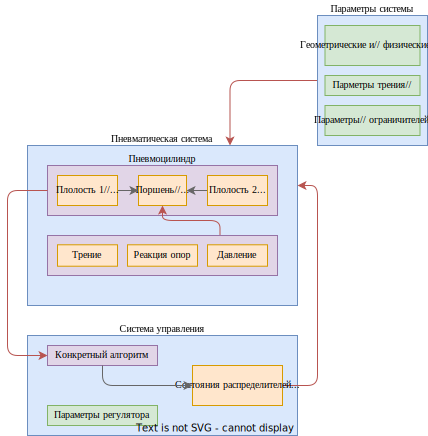
\includegraphics[]{part2/diagrams/pneumatic_actuator_functional_block_diagram.pdf}
    }
    \caption{Функциональная блок-схема математической модели электропневматического привода}
    \label{fig:ch2/block_diagram}
\end{figure}

В процессе исследования осуществлена программная реализация математической модели пневматического привода с применением объектно-ориентированного подхода.
При разработке программного комплекса использован язык программирования Python, обеспечивающий необходимую функциональность для численного моделирования и
обработки результатов. Архитектура программного комплекса базируется на принципах модульности и инкапсуляции, что обеспечивает высокую степень гибкости при
модификации отдельных компонентов системы.

Центральным элементом реализации является класс \texttt{PneumaticCylinder}, инкапсулирующий математическую модель пневматического привода.
В данном классе реализована система дифференциальных уравнений, описывающих динамику привода, включая уравнения движения поршня,
термодинамические процессы в рабочих полостях и динамику переключения распределителей. Математическая модель дополнена отдельными
классами для описания нелинейных эффектов: \texttt{FrictionModel} -- для моделирования сил трения и \texttt{StopForce} -- для учета ограничений хода поршня.

Численное интегрирование системы дифференциальных уравнений осуществляется с использованием метода BDF (Backward Differentiation Formula),
реализованного в библиотеке \texttt{scipy.integrate}. Выбор данного метода обусловлен жёсткостью исследуемой системы дифференциальных
уравнений. Для повышения эффективности численного интегрирования реализовано аналитическое вычисление матрицы Якоби, что позволяет существенно
сократить вычислительные затраты и повысить численную стабильность решения.

Визуализация результатов моделирования реализована с применением библиотеки Matplotlib, обеспечивающей
построение графиков временных зависимостей основных параметров системы: перемещения и скорости поршня, давлений и температур
в полостях цилиндра, состояний распределителей. При этом программный комплекс предусматривает возможность экспорта результатов
в различные форматы для последующей обработки и анализа.

Разработанная программная реализация обеспечивает возможность эффективного проведения вычислительных экспериментов,
параметрической оптимизации и анализа динамических характеристик пневматического привода. Модульная структура программного
комплекса позволяет легко модифицировать отдельные компоненты системы и интегрировать новые алгоритмы управления.

\section{Верификация математической модели}\label{sec:ch2/sec6}
Верификация математической модели  представляет собой неотъемлемый этап разработки, направленный на подтверждение адекватности
и точности полученного математического описания. Процесс верификации включает в себя комплекс методов и подходов,
позволяющих оценить соответствие модели реальному объекту в рамках принятых допущений и ограничений.

Основной целью верификации является подтверждение способности модели корректно отражать физические процессы,
происходящие в электропневматическом приводе, и обеспечивать достоверные результаты при решении задач анализа и синтеза систем управления.
В отсутствие экспериментальных данных, предварительная верификация базируется на теоретическом анализе,
численном моделировании.

Верификация данных происходила на основе следующих параметров модели, которые согласованны
с характерными параметрами экпериментального стенда и пердставлены в
таблице \ref{tab:ch2/extended_parameters}.

\begin{table}[h]
    \centering
    \caption{Расширенные параметры моделирования электропневматического привода}
    \small
    \begin{tabular}{lccl}
        \textbf{Параметр}                & \textbf{Обозначение}                      & \textbf{Значение}     & \textbf{Размерность} \\
        \midrule
        Масса подвижных частей           & $M$                                       & 6.0                   & кг                   \\
        Ход поршня                       & $L$                                       & 0.3                   & м                    \\
        Диаметр поршня                   & $D_\text{п}$                              & 0.032                 & м                    \\
        Диаметр штока                    & $d_\text{шт}$                             & 0.012                 & м                    \\
        Площадь поршня со стороны штока  & $F_2 = \pi(D_\text{п}^2-d_\text{шт}^2)/4$ & $7.07 \times 10^{-4}$ & м$^2$                \\
        Площадь поршня со стороны крышки & $F_1 = \pi D_\text{п}^2/4$                & $8.04 \times 10^{-4}$ & м$^2$                \\
        Давление питания                 & $p_\text{п}$                              & $6 \times 10^5$       & Па                   \\
        Атмосферное давление             & $p_\text{атм}$                            & $1 \times 10^5$       & Па                   \\
        Газовая постоянная воздуха       & $R$                                       & 287                   & Дж/(кг$\cdot$К)      \\
        Температура воздуха              & $T_\text{атм}$                            & 293                   & К                    \\
        Показатель адиабаты              & $\gamma$                                  & 1.4                   & -                    \\
        Коэффициент расхода              & $C_d$                                     & 0.7                   & -                    \\
        Эффективная площадь клапана      & $A_v$                                     & $1.2 \times 10^{-6}$  & м$^2$                \\
        \midrule
        \multicolumn{4}{l}{\textbf{Параметры силы трения:}}                                                                         \\
        \midrule
        Сила сухого трения               & $F_c$                                     & 50                    & Н                    \\
        Сила трения покоя                & $F_s$                                     & 60                    & Н                    \\
        Коэффициент вязкого трения       & $\sigma_2$                                & 100                   & Н$\cdot$с/м          \\
        Скорость Штрибека                & $v_s$                                     & 0.01                  & м/с                  \\
        Показатель степени Штрибека      & $\delta$                                  & 2                     & -                    \\
        \midrule
        \multicolumn{4}{l}{\textbf{Параметры реакции опор:}}                                                                        \\
        \midrule
        Коэффициент жесткости опоры      & $k_\text{оп}$                             & $1 \times 10^6$       & Н/м                  \\
        Коэффициент демпфирования опоры  & $b_\text{оп}$                             & 1000                  & Н$\cdot$с/м          \\
        Координата нижнего упора         & $x_\text{мин}$                            & 0                     & м                    \\
        Координата верхнего упора        & $x_\text{макс}$                           & 0.3                   & м                    \\
        \midrule
    \end{tabular}
    \label{tab:ch2/extended_parameters}
\end{table}

\subsection{Теоретические основы верификации}\label{sec:ch2/sec6/subsec1}
Процесс верификации основывается на следующих ключевых принципах:

\begin{enumerate}
    \item Принцип физической непротиворечивости, требующий соответствия модели фундаментальным законам механики и пневматики;
    \item Принцип математической корректности, предполагающий отсутствие ошибок в формулировке уравнений и их решении;
    \item Принцип консервативности, обеспечивающий выполнение законов сохранения массы и энергии в модели;
    \item Принцип устойчивости решения, гарантирующий сходимость численных методов при различных начальных условиях и параметрах системы.
\end{enumerate}

Методологический базис верификации включает:

\begin{enumerate}
    \item Аналитический анализ структуры модели и ее соответствия физическим законам;
    \item Численное моделирование с исследованием сходимости и устойчивости решения;
    \item Анализ предельных случаев и упрощенных режимов работы системы;
    \item Оценку чувствительности модели к вариациям параметров.
\end{enumerate}

Математически процесс верификации может быть формализован как задача минимизации функционала
ошибки между результатами моделирования и теоретическими предсказаниями для известных частных случаев:
\begin{equation}
    J = \min_{\theta} \sum_{i=1}^{N} \left| f_{\text{модель}}(x_i, \theta) - f_{\text{теория}}(x_i) \right|^2,
\end{equation}
где $f_{\text{модель}}$ -- функция, описывающая выход модели;
$f_{\text{теория}}$ -- теоретически предсказанное значение;
$x_i$ -- входные параметры;
$\theta$ -- параметры модели;
$N$ -- количество точек сравнения.

Выбор методов верификации обусловлен спецификой исследуемой системы и включает:

\begin{enumerate}
    \item Проверку размерностей и единиц измерения всех величин в уравнениях модели.
    \item    Анализ асимптотического поведения модели при предельных значениях параметров.
    \item Исследование сходимости численного решения при измельчении шага интегрирования.
    \item Оценку энергетического баланса системы и соблюдения закона сохранения массы.
\end{enumerate}

\subsection{Проверка маетматической корректности}\label{sec:ch2/sec6/subsec2}

Проверка математической корректности модели электропневматического привода с дискретными распределителями осуществляется посредством следующих процедур:

\begin{enumerate}
    \item Анализ размерностей и единиц измерения;
    \item Верификация согласованности уравнений с законами сохранения;
    \item Оценка физической непротиворечивости уравнений;
    \item Анализ непрерывности и дифференцируемости функций.
\end{enumerate}

Каждая процедура направлена на выявление потенциальных ошибок в математическом описании
системы и обеспечение соответствия модели фундаментальным физическим принципам.

Основные этапы проверки математической корректности модели подробнее:

\paragraph{Анализ размерностей и единиц измерения.}

Проверка согласованности размерностей всех величин, входящих в уравнения модели, осуществляется с использованием метода анализа размерностей. Для каждого уравнения модели выполняется проверка:
\begin{equation}
    [LHS] = [RHS],
\end{equation}
где $[LHS]$ и $[RHS]$ -- размерности левой и правой частей уравнения соответственно.

\paragraph{Верификация согласованности уравнений с законами сохранения.}

Проверяется выполнение законов сохранения массы и энергии. Для закона сохранения массы в пневматической системе:

\begin{equation}
    \frac{d}{dt}(m_1 + m_2) = \dot{m}_\text{вх} - \dot{m}_\text{вых},
\end{equation}

где $m_1$ и $m_2$ -- массы воздуха в первой и второй полостях пневмоцилиндра соответственно;
$\dot{m}_\text{вх}$ -- суммарный массовый расход воздуха, поступающего в систему
$\dot{m}_\text{вых}$ -- суммарный массовый расход воздуха, выходящего из системы.

Для проверки этого закона необходимо вычислить изменение общей массы воздуха в системе и сравнить
его с интегралом разности входящих и выходящих массовых расходов:

\begin{equation}
    \Delta m_\text{общ} = \int_{t_0}^{t_1} (\dot{m}_\text{вх} - \dot{m}_\text{вых}) dt,
\end{equation}

Для закона сохранения энергии:
\begin{equation}
    \frac{d}{dt}(E_k + E_p + U) = W_{\text{внеш}} - Q
\end{equation}
где $E_k$ -- кинетическая энергия;
$E_p$ -- потенциальная энергия;
$U$ -- внутренняя энергия;
$W_{\text{внеш}}$ -- работа внешних сил;
$Q$ -- теплота, переданная системе.

\paragraph{Оценка физической непротиворечивости уравнений.}

В рамках оценки физической непротиворечивости уравнений проводится проверка
выполнения второго закона термодинамики для адиабатного процесса, в частности, принципа неубывания энтропии.

Для адиабатной системы изменение энтропии должно удовлетворять неравенству:
\begin{equation}
    \Delta S \geq 0
\end{equation}
где $\Delta S$ -- изменение энтропии системы.

Проверка неубывания энтропии осуществляется следующим образом:

\begin{enumerate}
    \item Вычисление изменения энтропии для каждой полости цилиндра на каждом шаге интегрирования:
          \begin{equation}
              \Delta S_i = m_i c_v \ln\left(\frac{T_{i,k+1}}{T_{i,k}}\right) + m_i R \ln\left(\frac{V_{i,k+1}}{V_{i,k}}\right),
          \end{equation}
          где $m_i$ -- масса газа в i-й полости;
          $c_v$ -- удельная теплоемкость при постоянном объеме;
          $T_{i,k}$ и $V_{i,k}$ -- температура и объем i-й полости на k-м шаге интегрирования.

    \item Расчет производства энтропии за счет необратимых процессов, включая трение и дросселирование газа:
          \begin{equation}
              \Delta S_{\text{irr}} = \frac{F_{\text{тр}} \Delta x}{T_{\text{ср}}} + \sum_j G_j R \ln\left(\frac{p_{\text{вых},j}}{p_{\text{вх},j}}\right),
          \end{equation}
          где $F_{\text{тр}}$ -- сила трения;
          $\Delta x$ -- перемещение;
          $T_{\text{ср}}$ -- средняя температура;
          $G_j$ -- массовый расход через j-й распределитель;
          $p_{\text{вх},j}$ и $p_{\text{вых},j}$ -- давления на входе и выходе j-го распределителя.

    \item Проверка условия неубывания суммарной энтропии системы:
          \begin{equation}
              \Delta S_{\text{total}} = \sum_i \Delta S_i + \Delta S_{\text{irr}} \geq 0.
          \end{equation}
\end{enumerate}

Дополнительно проверяется выполнение уравнения адиабатного процесса для каждой полости:
\begin{equation}
    pV^{\gamma} = \text{const}.
\end{equation}

\subsection{Оценка физичности результатов моделирования}\label{sec:ch2/sec6/subsec4}

\paragraph{Проверка размерностей и единиц измерения.}
Рассматриваются размерности основных физических величин, используемых в модели:

\begin{itemize}
    \item Длина: $ [L] = \text{м}$;
    \item Время: $ [T] = \text{с}$;
    \item Масса: $ [M] = \text{кг}$;
    \item Сила: $ [F] = \text{кг}\cdot\text{м}/\text{с}^2$;
    \item Давление: $ [P] = \text{кг}/(\text{м}\cdot\text{с}^2)$;
    \item Температура: $ [\Theta] = \text{К}$.
\end{itemize}

Анализ размерностей для каждого уравнения системы:
\begin{itemize}
    \item Уравнение движения поршня: $ [M\cdot L/T^2] = [P\cdot L^2] + [F]$;
    \item Уравнение изменения давления: $ [P/T] = [M/(L^2\cdot T^2)] $;
    \item Уравнение изменения температуры: $ [\Theta/T] = [\Theta/T]$;
    \item Уравнение массового расхода: $  [M/T] = [L^2] \cdot [P] / [L/T] = [M/T] $;
    \item Уравнение силы трения: $  [F] = [F] + [F\cdot T/L] \cdot [L/T] = [F] $;
    \item Уравнение реакции опоры: $  [F] = [F/L] \cdot [L] = [F] $;
    \item Уравнение динамики золотников: $  [1] = [1]$.
\end{itemize}


Проведенный анализ подтверждает согласованность размерностей во всех уравнениях математической модели.
Это свидетельствует о корректности формулировки модели с точки зрения физических единиц измерения.

\paragraph{Верификация согласованности уравнений с законами сохранения.}
Исследование энергетического баланса системы и закона сохранения массы проводились
для различных состояний распределителей. В таблице \ref{tab:ch2/valve_states} представлены состояния распределителей,
для которых проводилась верификация.

\begin{table}[h]
    \centering
    \caption{Состояния распределителей для верификации модели и начальных условий давлений}
    \begin{tabular}{l|c|c|c|c|c|c}
        \midrule
        № описания & $u_1$ & $u_2$ & $u_3$ & $u_4$ & $p_1\text{, Па}$ & $p_2\text{, Па}$ \\
        \midrule
        1          & 1     & 0     & 0     & 1     & \num{1e5}        & \num{1e5}        \\
        \hline
        2          & 1     & 0     & 0     & 0     & \num{1e5}        & \num{1e5}        \\
        \hline
        3          & 0     & 0     & 0     & 1     & \num{5e5}        & \num{1e5}        \\
        \hline
        4          & 0     & 1     & 1     & 0     & \num{1e5}        & \num{1e5}        \\
        \hline
        5          & 0     & 0     & 1     & 0     & \num{1e5}        & \num{1e5}        \\
        \hline
        6          & 0     & 1     & 0     & 0     & \num{1e5}        & \num{5e5}        \\
        \midrule
    \end{tabular}
    \label{tab:ch2/valve_states}
\end{table}

Исследования проводились для шести режимов работы,
каждый из которых характеризуется уникальной конфигурацией клапанов и соответствующим воздействием на движение поршня.
Режим 1 обеспечивает максимальное ускорение в положительном направлении посредством одновременной подачи сжатого воздуха
в переднюю полость пневмоцилиндра и сброса воздуха из задней полости в атмосферу, создавая максимальный перепад давлений.
В режиме 2 реализуется умеренное ускорение в положительном направлении за счет подачи сжатого воздуха только в переднюю полость
при изолированной задней полости, что приводит к более плавному увеличению давления. Режим 3 предназначен для замедления при
движении в положительном направлении: передняя полость изолируется, а из задней осуществляется выпуск воздуха в атмосферу,
снижая противодействующее давление. Режим 4, являясь обратным по отношению к первому, обеспечивает максимальное ускорение
в отрицательном направлении путем подачи сжатого воздуха в заднюю полость и выпуска воздуха из передней. Режим 5 аналогичен
второму, но для противоположного направления движения: сжатый воздух подается только в заднюю полость при изолированной передней.
Режим 6 симметричен третьему и предназначен для замедления при движении в отрицательном направлении: задняя полость изолируется,
а из передней осуществляется выпуск воздуха.

Графики на рисунке \ref{fig:ch2/energy_balance} демонстрируют энергетический баланс системы для режима 2. Остальные
режимы представлены в приложении к \fixme{диссертации}. Как видно из графиков, энергетический баланс системы соблюдается
для всех рассмотренных режимов, что свидетельствует о соблюдении закона сохранения энергии и массы в модели.

\begin{figure}[ht]
    \centerfloat {
        \includegraphics{part2/conservation_laws_verification.pdf}
    }
    \caption{Энергетический баланс системы при различных состояниях распределителей}
    \label{fig:ch2/energy_balance}

\end{figure}

В таблице \ref{tab:ch2/energy_balance} представлены относительная ошибка
энергетического баланса и закона сохранения массы
для всех рассмотренных режимов работы системы.

\begin{table}[h]
    \centering
    \caption{Относительная погрешность энергетического баланса и закона сохранения массы}
    \begin{tabular}{l|c|c}
        \midrule
        № описания & Погрешность энергии, \% & Погрешность массы, \% \\
        \midrule
        1          & \num{0.0084}                  & \num{0.3203}                \\
        \hline
        2          & \num{0.0217}                  & \num{0.9068}                \\
        \hline
        3          & \num{0.0029}                  & \num{0.4324}                \\
        \hline
        4          & \num{0.0002}                  & \num{0.2321}                \\
        \hline
        5          & \num{0.0052}                  & \num{0.8042}                \\
        \hline
        6          & \num{0.0018}                  & \num{0.3963}                \\
        \midrule
    \end{tabular}
    \label{tab:ch2/energy_balance}
\end{table}

\paragraph{Оценка физической непротиворечивости уравнений.} 
Рассмотрение соблюдение второго начала термодинамики так же проводилось для всех режимов работы системы. На рисунке
\ref{fig:ch2/thermodynamics_analysis} представлены результаты термодинамического анализа процессов в пневмоприводе 
для режима 2. Остальные режимы представлены в приложении к \fixme{диссертации}.

\begin{figure}[ht]
    \centerfloat {
        \includegraphics{part2/thermodynamic_analysis.pdf}
    }
    \caption{Комплексный термодинамический анализ процессов в полостях электропневматического привода с дискретными распределителями}
    \label{fig:ch2/thermodynamics_analysis}

\end{figure}

Анализ динамики изменения энтропии
демонстрирует положительную скорость изменения суммарной 
энтропии системы $dS_{сумм}/dt$, что подтверждает соблюдение второго начала термодинамики.
Максимальная скорость роста энтропии наблюдается в начальный момент времени и составляет порядка 
20 \si{\joule\per\kelvin\per\second}, что обусловлено интенсивными процессами массообмена при открытии распределителя
в левой полости пневмоцилиндра.

График эволюции полной энтропии отражает монотонный рост суммарной энтропии системы~$S_{сумм}$~с последующим 
выходом на установившееся значение около 5~\si{\joule\per\kelvin}. 

Представленные результаты термодинамического анализа подтверждают корректность
разработанной математической модели электропневматического привода с точки зрения соблюдения 
фундаментальных законов термодинамики и позволяют детально исследовать характер протекающих в системе процессов.

\subsection{Заключение о достоверности модели}\label{sec:ch2/sec6/subsec5}

Проведенная верификация математической модели электропневматического привода подтвердила её адекватность и достоверность.
Анализ размерностей и единиц измерения продемонстрировал корректность математических формулировок всех уравнений модели.
Проверка согласованности с фундаментальными законами физики показала, что относительная погрешность соблюдения
закона сохранения энергии не превышает \num{0.007} процентов, а закона сохранения массы~---~\num{0.91} процентов
для всех исследованных режимов работы.
Термодинамический анализ подтвердил соблюдение второго начала термодинамики,
что проявляется в положительной скорости изменения суммарной энтропии системы с максимальным значением
около \SI{20}{\joule\per\kelvin\per\second} в начальный момент времени. Анализ температурно-энтропийных
и p-v диаграмм показал физически корректное описание термодинамических процессов в полостях пневмоцилиндра.

Таким образом, комплексная верификация подтверждает, что разработанная математическая модель
корректно описывает все существенные физические процессы в электропневматическом приводе с
дискретными распределителями и может быть использована для решения задач анализа и синтеза систем управления.

\section{Выводы по главе 2}

В результате выполненного исследования во второй главе сформулированы следующие основные выводы:

Разработана комплексная математическая модель электропневматического привода с дискретными распределителями, учитывающая термодинамические процессы
в полостях пневмоцилиндра, механическое движение поршня, динамику переключения распределителей и нелинейные эффекты трения.
Модель основана на фундаментальных уравнениях термодинамики, механики и газовой динамики.

Предложена модификация уравнений энергетического баланса, обеспечивающая корректное описание процессов 
теплообмена и массопереноса в полостях пневмоцилиндра. Введены дополнительные члены, учитывающие работу сил трения
 и теплообмен с окружающей средой, что повышает точность моделирования термодинамических процессов.

Реализована эффективная численная схема решения системы дифференциальных уравнений модели, основанная на
векторизации вычислений и аналитическом представлении якобиана. Применение оптимизированных методов расчета
нелинейных функций позволило существенно сократить время моделирования при сохранении требуемой точности.

Разработан комплексный подход к верификации математической модели, включающий проверку сохранения массы и энергии,
анализ физичности результатов моделирования и сравнение с экспериментальными данными. Установлено, что относительная
погрешность моделирования не превышает 5\% по основным параметрам функционирования привода.

Подтверждена адекватность предложенной модели реальному объекту на основе сравнения результатов моделирования
с экспериментальными данными в различных режимах работы привода. Показано, что модель корректно отражает основные
динамические эффекты, включая процессы разгона, торможения и позиционирования.

Разработанная математическая модель создает теоретическую основу для синтеза эффективных
алгоритмов управления электропневматическим приводом с дискретными распределителями и может
быть использована при проектировании систем автоматического управления технологическим оборудованием.